\documentclass[handout]{beamer}

\usepackage[utf8]{inputenc}
\usepackage[polish]{babel}
\usepackage[T1]{fontenc}
\usepackage{amsfonts}
\usepackage{amsthm}
\usepackage{amsmath}
\usepackage{amssymb}
\usepackage{mathabx}
\usepackage{array}             
\usepackage{dsfont}
\usepackage{url}
\usepackage{wrapfig}
\usepackage{subcaption}
\usepackage{blkarray}
\usepackage{opensans}
\usepackage{float}
\usepackage{xspace}
\usepackage{xcolor}
\usepackage{hyperref}
\usepackage{algorithm}
\usepackage[noend]{algpseudocode}
\def\Z{\mathbb Z}
\def\Q{\mathbb{Q}}
\def\A{\mathbb{A}}

\usepackage{listings}
\usepackage{ bbold }

\hypersetup{
    colorlinks=true,
    linkcolor=blue,
    filecolor=magenta,      
    urlcolor=blue,
}

%Information to be included in the title page:
\title{Problem Skolema -- LATO proseminar}
\author{Marcin Wierzbiński}
\institute{MIMUW}
\date{\today}


\theoremstyle{definition}
\newtheorem*{definicja}{Definicja}
\newtheorem*{twierdzenie}{Twierdzenie}
\newtheorem*{uwaga}{Uwaga}
\newtheorem*{lemat}{Lemat}
\newtheorem*{przyklad}{Przykład}


\newtheoremstyle{named}{}{}{\itshape}{}{\bfseries}{.}{.5em}{\thmnote{#3's }#1}
\theoremstyle{named}
\newtheorem*{namedtheorem}{Twierdzenie}



\begin{document}
\frame{\titlepage}

\begin{frame}{Motywacja}
\begin{itemize}
    \item Twierdzenie Skolema dla RLR rzędu $2$
    \item Problem Skolema i teoria automatów
\end{itemize}
\end{frame}
% tlumaczenie dlaczego to nie jest wykonywalna na maszynie

\begin{frame}{Zacznijmy od prostego programu}
    \begin{algorithm}[H] 
        \begin{algorithmic}[l]
        \State $\vec{x} := \vec{a}, \quad \vec{a} \in \Z^{k}$  \algorithmiccomment{Wejście}
        \While { $u^{T}\cdot \vec{x} \neq 0$ }
          \State $\vec{x} := M \vec{x}$ \algorithmiccomment{$M \in \Z^{k \times k}$}
          
        \EndWhile
        \end{algorithmic}
    \end{algorithm}
    
    \begin{itemize}
    \pause 
    \item Jestem zainteresowany problemem stopu dla tego problemu? 
    
    
    \item  Zakładamy nieskończona pamięć, ponieważ $\vec{x}$ może rosnąć bardzo szybko do nieskończoności, np przy $M=2$
    \pause
    
    \item  Czy jest rozstrzygalny ten program? Kto twierdzi inaczej?
    \end{itemize}

\end{frame}

\begin{frame}{Pytanie o inny warunek}
    Zmieńmy warunek na inny 
    \begin{algorithm}[H] 
        \begin{algorithmic}[l]
        \State $\vec{x} := \vec{a},  \quad \vec{a} \in \Z^{k}$  \algorithmiccomment{Wejście}

        \While { $u^{T}\cdot \vec{x} \geq 0$ }
          \State $\vec{x} := M \vec{x}$ \algorithmiccomment{$M \in \Z^{k \times k}$}
          
        \EndWhile
        \end{algorithmic}
    \end{algorithm}
\end{frame}    

\begin{frame}{Inne pytanie z terminów automatów}
    Mamy alfabet $\Sigma$  oraz A, B skończony automat deterministyczny nad $\Sigma$
    \begin{itemize}
        \item $u_n$ jest numerem słów długości $n$ akceptowanych przez $A$
        \item  $v_n$ jest numerem slow długości $n$ akceptowanych przez $B$

    \end{itemize}
    Pytanie:
    \begin{itemize}
        \item  Czy istnieje $n$ takie, że ilość słów akceptowanych przez $A$ jest równa ilości słów akceptowanych przez $B$ 
        \item  Nie wiemy, czy ten problem jest rozstrzygalny ani nierozstrzygalny. 
    \end{itemize}
    \pause
    
    Znana jest rozstrzygalność dla automatów rozmiaru $4$

\end{frame}

\begin{frame}{Równoważność pytania -- przykład}
    \begin{figure}
        \centering
        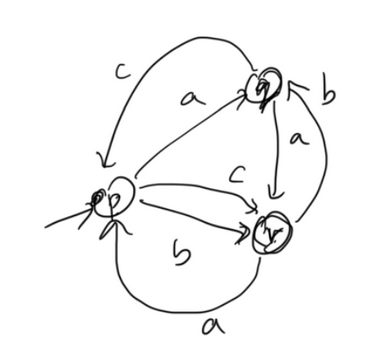
\includegraphics[width=40mm]{img/Zaznaczenie_079.png}
        \caption{Automat skończony ze stanami $p, g, r$ i alfabetem $\Sigma = \{a,b,c \}$}
        \label{fig:my_label}
    \end{figure}
    \begin{cases}
        p_{n+1} = r_n + g_n \\
        g_{n+1} = p_n + r_n \\ 
        r_{n+1} = 2 p_n + q_n \\ 
        (p_0, q_0, r_0) = (1,0,0) 
    \end{cases}
\end{frame}

\begin{frame}{Macierz przejścia dla automatu}
\begin{figure}
    \centering
    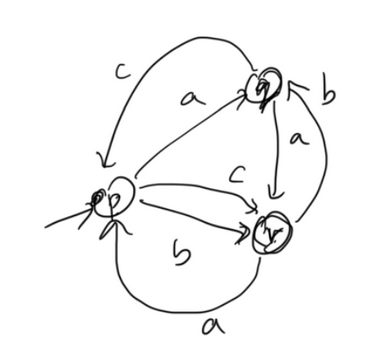
\includegraphics[width=40mm]{img/Zaznaczenie_079.png}
    \caption{Automat skończony ze stanami $p, g, r$ i alfabetem $\Sigma = \{a,b,c \}$}
    \label{fig:my_label}
\end{figure}
    $$
    (p_{n+1}, q_{n+1}, r_{n+1}) 
    = (p_{n},q_{n},r_{n}) \begin{bmatrix}
    0 & 1 & 2 \\
    1 & 0 & 1 \\
    1 & 1 & 0
    \end{bmatrix}
    $$
\end{frame}

\begin{frame}{Liniowe równanie rekurencyjne}
    $$
        a_0, \ldots a_{k-1} \in \mathbb{Z} 
    $$

    $$
        u_0, \ldots, u_{k-1} \in \mathbb{Z}
    $$


    Liniowe równanie rekurencyjne: 
    $$
    u_{n+k}=a_{1} u_{n+k-1}+a_{2} u_{n+k-2}+\ldots+a_{k} u_{n}
    $$
    Zwykłe oznaczenie $\large u_n \rarge _{n=1}^{\infty}$
    $a_0 \neq 0$
\end{frame}


\begin{frame}{Równoważność pytania -- przykład}
Weźmy dwa ciągi rekurencyjne liniowe $f_n, g_n$
    \begin{equation*}
        f_{n} = [1,0] \begin{bmatrix}
            1 & 1 \\
            0 & 1 
        \end{bmatrix}^{n}
        \begin{bmatrix}
            1 & 0
        \end{bmatrix}
    \end{equation*}
    \begin{equation*}
         g_{n} = [2,5] \begin{bmatrix}
            3 & 2 \\
            0 & -1 
        \end{bmatrix}^{n}
        \begin{bmatrix}
            2 & -1
        \end{bmatrix}
    \end{equation*}
    
    \begin{align*}
        u_n = f_n - q_n && \text{jest ciągiem rekurencyjnym} 
    \end{align*}
    $$
        f_n - g_n = [1,0|2,5] 
        \left[
        \begin{array}{cc|cc}
        1 & 1 & 0 & 0 \\
        0 & 1 & 0 & 0 \\
        \hline
        0 & 0 & 3 & 2 \\
        0 & 0 & 0 & -1
        \end{array}
        \right]
        \begin{bmatrix}
            1  \\
            0  \\
            \hline
            -2 \\
            1 
        \end{bmatrix}
    $$
    
\end{frame}

\begin{frame}
    Przykład:
    Równanie Fibonacciego:
   \begin{equation*}
        \begin{cases}
        u_{n+2} = u_{n+1} + u_n \\
        u_{1} = 1 \\
        u_{0} = 0
        \end{cases}
    \end{equation*}
    Jest bliska styczność z przykładami wyżej. 

\end{frame}

\begin{frame}{Zapis macierzowy}
    $$\exist v, w \in \mathbb{Z}^{k}, M \in \mathbb{Z}^{k\times k} $$
    $$u_n = v^{t}M^{n}w$$

    $$
    M = \begin{bmatrix}
    a_{k-1} & 1 &  \ldots & 0 \\
    a_{k-2} & 0 & 1 & \ldots 0  \\
    \vdots & 0 & \ldots & 0 \\ 
    a_1 & 0 & \ldots & 1 \\
    a_0 & 0 & \ldots & 0
    \end{bmatrix}
    $$
\end{frame}

\begin{frame}{Równanie Fibonacciego:}
\begin{equation*}
\begin{cases}
u_{n+2} = u_{n+1} + u_n \\
u_{1} = 1 \\
u_{0} = 0 
\end{cases}
\end{equation*}
\begin{equation*}
        \begin{bmatrix}
        u_{n+2} & u_{n+1} \\
        u_{n+1} & u_{n} 
        \end{bmatrix} 
        \cdot
        \begin{bmatrix}
        1 & 1\\
        1 & 0
        \end{bmatrix}
        = 
        \begin{bmatrix}
        u_{n+3} & u_{n+2}\\
        u_{n+2} & u_{n+1}
        \end{bmatrix}
\end{equation*}
Ponieważ równocześnie:
\begin{equation*}
    \begin{bmatrix}
    1 & 1 \\
    1 & 0 
    \end{bmatrix}= 
    \begin{bmatrix}
    u_2 & u_1 \\
    u_1 & u_0
    
    \end{bmatrix}
\end{equation*}
to indukcyjnie: 
\begin{table}[]
    \centering
    \begin{tabular}{c|c}
       \begin{equation*}
    
        \begin{bmatrix}
        1 & 1\\
        1 & 0
        \end{bmatrix}^n
        = 
        \begin{bmatrix}
        u_{n+1} & u_n\\
        u_{n} & u_{n-1}
        \end{bmatrix}

    \end{equation*}
&  
       \begin{equation*}
        \begin{bmatrix}
        u_{n+1} \\
        u_{n}
        \end{bmatrix}
        = 
        \begin{bmatrix}
        1 & 1\\
        1 & 0
        \end{bmatrix}^n
        \begin{bmatrix}
        u_1 \\
        u_0 
        \end{bmatrix}

    \end{equation*}

    \end{tabular}
\end{table}


\end{frame}

\begin{frame}{Lemat redukcji}

\begin{namedtheorem}[Cayleya-Hamiltona]
    Jeśli $p(t)$ jest wielomianem charakterystycznym dla macierzy $M$, wtedy macierz $p(M)$ jest macierzą zerową. 
\end{namedtheorem}

\begin{twierdzenie}

    Niech $v, w \in \Z^{k}, M \in \Z^{k\times k}$ oraz $u_n = v^{t}M^{n}w \in \Z$
    
    Niech
    \begin{table}[]
        \centering
        \begin{tabular}{c|c}
    $
    M = \begin{bmatrix}
    a_{1} & 1 &  \ldots & 0 \\
    a_{2} & 0 & 1 & \ldots 0  \\
    \vdots & 0 & \ldots & 0 \\ 
    a_{k-1} & 0 & \ldots & 1 \\
    a_{k} & 0 & \ldots & 0
    \end{bmatrix}
    $
             &  
    $v= \begin{bmatrix}
    u_{k-1} \\ u_{k-2} \\ \vdots \\ u_{0} \\
    \end{bmatrix}
    w =  \begin{bmatrix}
    0 \\ 0 \\ \vdots \\ 1 \\
    \end{bmatrix}
    $
             & 
        \end{tabular}

    \end{table}
    
    Wtedy i tylko wtedy $\<u_n\>$ jest liniowym równaniem rekurencyjnym. 

\end{twierdzenie}

\end{frame}

\begin{frame}{Twierdzenie c.d}

\begin{proof}
    Weźmy $M$ wówczas z twierdzenia CH: 
    \begin{equation}
        M^{k} =  a_1 M^{k} + \ldots a_0 \mathbb{1} \
    \end{equation}
    może to równanie przez 
    \begin{equation}
        v^{t}M^{k} = a_1 v^{t} M^{k-1} + \ldots a_k v^{t} \mathbb{1} 
    \end{equation} 


i domnażam przez $M^{n}$ z lewej strony 
      \begin{equation}
          v^{t}M^{k} M^{n} = a_1 v^{t} M^{k-1} M^{n} + \ldots a_k v^{t} \mathbb{1} M^{n}
      \end{equation}
      i pomnażam 
      $$ v^{t}M^{k + n} w = a_1 v^{t} M^{k-1 + n}w + \ldots a_k v^{t} M^{n}w $$ 
      co daję tezę
\end{proof}
\end{frame}

\begin{frame}{Twierdzenie w drugą stronę}
\begin{proof}
    Niech $<u_n>$ będzie równaniem liniowym rekurencyjnym z warunkiem początkowym:
    $u_{n+k} = a_1 u_{n+k-1} + \ldots a_{k} u_{k}$
    przez indukcje pokazuje się, że $u_{n} = v^{t}M^{n}w $
    
    Sprawdźmy bazę indukcyjną:
    $n=0$
    
    wtedy $u_{0} = v^{t} \mathbb{1} w = u_0$
    
\end{proof}
\end{frame}



\begin{frame}{Równania rekurencyjne}
Równanie rekurencyjne Fibonacciego: 
$$
{\displaystyle u_{n}={\frac {1}{\sqrt {5}}}\left({\frac {1+{\sqrt {5}}}{2}}\right)^{n}-{\frac {1}{\sqrt {5}}}\left({\frac {1-{\sqrt {5}}}{2}}\right)^{n}.}
$$
 Jak zapisać za pomocą równania rekurencyjnego? 
\begin{itemize}
    \item  $u_n = n$
    \pause 
    \item $u_n = u_{n-1} + 1$
    \pause
    \item  $u_n = n^{2}$
    \pause
    \item $u_n = 3 u_{n+2} - 3u_{n+1} + u_n$

\end{itemize}

\end{frame}

\begin{frame}{Dekompozycja dla Fibonacciego}
    \begin{equation*}
        \begin{bmatrix}
        u_{n+1} \\
        u_{n}
        \end{bmatrix}
        = 
        \begin{bmatrix}
        1 & 1\\
        1 & 0
        \end{bmatrix}^n
        \begin{bmatrix}
        u_1 \\
        u_0 
        \end{bmatrix}

    \end{equation*}
    Liczymy rozkład $M = PDP^{-1}$ i uzyskujemy $\lambda_1 =  \frac{1}{2} \left(1-\sqrt{5}\right), \lambda_2 = \frac{1}{2} \left(1-\sqrt{5}\right) $
\begin{equation*}
    u_n = 
        \begin{bmatrix}
           1 & 0
        \end{bmatrix}
        \begin{bmatrix}
            \lambda_1 & \lambda_2 \\
         1 & 1 \\
        \end{bmatrix}
        \begin{bmatrix}
           \lambda_1^{n} & 0 \\
            0 & \lambda_2^{n}
        \end{bmatrix}
        \frac{1}{\sqrt{5}}
        \begin{bmatrix}
           1 & \lambda_2 \\
           -1  & \lambda_1 \\
        \end{bmatrix} 
        \begin{bmatrix}
           1 \\
           0
        \end{bmatrix}
    \end{equation*}
    \begin{equation*}
        u_n = \frac{\lambda_1^{n} - \lambda_2^{n}}{\sqrt{5}}
    \end{equation*}
 
 
\end{frame}

\begin{frame}{Liczby algebraiczne}
\begin{definicja}
    Powiemy, że $a $ jest liczbą algebraiczną, jeżeli jest pierwiastkiem niezerowego wielomianu $p \in \Q[x]$. 
\end{definicja}

\begin{przyklad}
    Liczba $\sqrt{2}$ jest liczbą algebraiczną wielomianu $p(x) = x^{2} - 2$
\end{przyklad}

\begin{definicja}
    Stopniem liczby algebraicznej 
\end{definicja}

\end{frame}


\begin{frame}{Problem Skolema dla równania rzędu 2}


\begin{twierdzenie}
    Niech $u_n$ jest równaniem rekurencyjnym liniowym rzędu 2
    $$
        u_n = c_1 u_{n+1} + c_2 u_n
    $$
    $$
        c_1, c_2 \in \mathbb{Q}
    $$
    $$
        u_0, u_1 \in \mathbb{Q}
    $$
    wówczas $\exists n : u_n = 0$
\end{twierdzenie}

\end{frame}

\begin{frame}{$\lambda_1= \lambda_2$}

\begin{proof}
    $$u_n = 0 \iff  u_n = a n \lambda^{n} + b \lambda^{n} = 0$$
    
    $$ a n \lambda^{n} + b \lambda^{n} = 0 $$
    $$ a n + b = 0 $$
    Rozwiązywalne dla $a, b \in \A \cap \Q $
\end{proof}

    
\end{frame}

\begin{frame}{Szkic dowodu $\lambda_1 \neq \lambda_2$}
    rozpatrzymy przypadek:
    $|\lambda_1| > |\lambda_2|, \lambda_1, \lambda_2 \in \mathbb{R}$
    
    Otrzymujemy wielomian charakterystyczny 
    $$
       a_1 \lambda^{n} = - a_2 \lambda^{n}
    $$
    $$
        - \frac{a_1}{a_2} = (\frac{\lambda_2}{\lambda_1})^{n}
    $$
    Poniżej pewnego $n$ nie ma szans na równość $\frac{\lambda_2}{\lambda_1}$
\end{frame}

\begin{frame}{$|\lambda_1| = |\lambda_2|$}

\begin{equation*}
    u_n = a \lambda^{n} + \overline{a} \overline{\lambda}^{n} 
\end{equation*}
\pause 
\begin{equation*}
    u_n = 0 
\end{equation*}
\pause 
\begin{equation*}
    a \lambda^{n} + \overline{a} \overline{\lambda}^{n} = 0 \iff Re(a {\lambda^{n}}) = 0 
\end{equation*} 
\pause
Weźmy: 
\begin{align*}
    v = \frac{\lambda}{|\lambda|} && |v| = 1
\end{align*}
$$\frac{u_n}{|\lambda|^{n}} = 0 \iff u_n = 0$$

\end{frame}
    
\begin{frame}{$|\lambda_1| = |\lambda_2|$}
\begin{table}[]
    \centering
    \begin{tabular}{c c}
       \begin{figure}
            \centering
            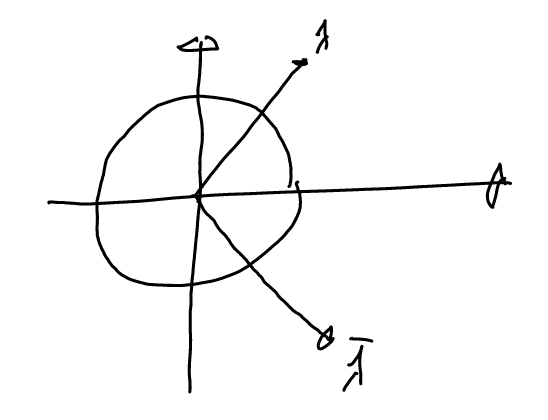
\includegraphics[width=40mm]{img/Zaznaczenie_081.png}
        \end{figure}  & 
            $\frac{u_n}{|\lambda|^n} = a v^{n} + \overline{a} \overline{v} ^{n} $
 
    \end{tabular}
\end{table}

\begin{equation*}
    a v^{n} \quad  \text{zanika na osi urojonej} \iff u_n = 0 \iff 
\end{equation*}
\begin{align*}
    v^{n} = \frac{i c}{a} && \text{gdzie} \quad |\frac{c}{a}| = 1
\end{align*}
\begin{align*}
    v^{n} = \beta && \text{gdzie $\beta$ jest pewną liczbą algebraiczną o module 1}
\end{align*}
\pause
Potrzebujemy rozwiązać równanie $v^{n} = \beta, v, \beta \in \A$

\end{frame}

\begin{frame}{Reprezentacja liczb algebraicznych }
    Mamy wielomian $p(x) = a_0 + a_1 x + \ldots x_{t} x^{t}$ stopnia $t$, niech $\alpha$ będzie jedynym pierwiastkiem  
    \begin{figure}
        \centering
        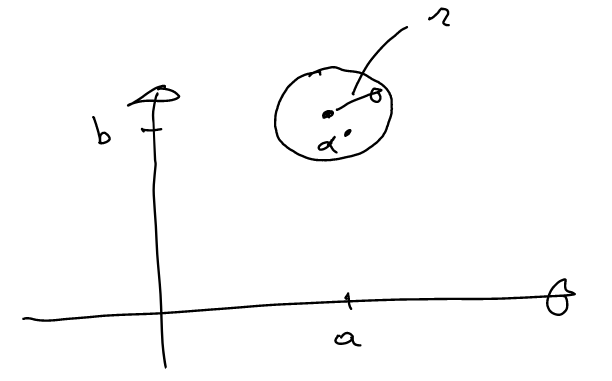
\includegraphics[width=40mm]{img/Zaznaczenie_082.png}
        \caption{Otoczenie liczby algebraicznej}
        \label{fig:my_label}
    \end{figure}
    $$H(P) = \max \{ |a_0|, \ldots, |a_t| \}$$
    \begin{twierdzenie}[Mignotte]
            Jeśli $a,b \in \A$ są różnymi pierwiastkami wielomianu $p$ wtedy 
            $|\alpha - \beta| > \frac{\sqrt{6}}{d^{\frac{d+1}{2}} H^{d-1}}$
    \end{twierdzenie}
    
\end{frame}


\begin{frame}{liczba całkowita algebraiczna}
    \begin{definicja}
        Liczbą \textbf{całkowitą algebraiczną} nazywamy pierwiastek wielomianu $p \in \Z[x]$ o współczynnikach całkowitych. Główny współczynnik wielomianu $p(x)$ jest równy 1. 
    \end{definicja}
    Wprowadźmy oznaczenie $O$ na pierścień liczb algebraicznych. Mamy pierścień z jednoznacznością rozkładu. 
\end{frame}

\begin{frame}{Frame Title}
    
\end{frame}


\begin{frame}


\begin{itemize}
    \item https://terrytao.wordpress.com/2007/05/25/open-question-effective-skolem-mahler-lech-theorem/
\end{itemize}
\end{frame}

\end{document}